%% LyX 2.2.1 created this file.  For more info, see http://www.lyx.org/.
%% Do not edit unless you really know what you are doing.
\documentclass[12pt,english]{article}
\usepackage[T1]{fontenc}
\usepackage[latin9]{inputenc}
\usepackage{geometry}
\geometry{verbose,tmargin=2cm,bmargin=2cm,lmargin=2cm,rmargin=2cm}
\usepackage{fancyhdr}
\pagestyle{fancy}
\usepackage{wrapfig}
\usepackage{calc}
\usepackage{amsmath}
\usepackage{amssymb}
\usepackage{graphicx}
\usepackage{esint}

\makeatletter

%%%%%%%%%%%%%%%%%%%%%%%%%%%%%% LyX specific LaTeX commands.
%% Because html converters don't know tabularnewline
\providecommand{\tabularnewline}{\\}

\makeatother

\usepackage{babel}
\begin{document}

\section{Introduction}

\textbf{\small{}The goal is to create an operational wildland fire
model that captures fireline behaviors that have been observed in
other models and experiments at a much smaller computational cost. }{\small \par}

Wildfires are multiscale systems with complex dynamics and feedback
mechanisms, making it difficult to capture all of their characteristics.
Physics based models, such as HIGRAD/FIRETEC \cite{linn1997firetec}
(H/F), model the fluid dynamics, the fire-atmosphere interaction,
and the chemical processes (pyrolysis) of fires. These models can
simulate a wide range of conditions but come with large computational
costs and highly complex initialization. This means these models do
not lend themselves to be used for exploring the development of a
fire under slightly varying conditions without a considerable investment
of time. Current operational fire models, used to forecast development
of active fires, are mostly based off the Rothermel spread model,
an empirical model originally developed in 1972. The Rothermel model
has The aim of this research is to develop models that are 

\section{Interface Tracking Model}

We cast the modeling of fire as an interface tracking problem where
a fireline is represented as either a single closed curve (entire
interior burning) ,$\Gamma_{0}$, or as an outer fireline with one
or multiple inner firelines (regions of exhausted or unburnt fuel),
$\Gamma_{i}$ for $i\geq1$. We assume that any burning section of
fuel can be encapsulated with a somewhat smooth continuous curve.
The firelines, $\Gamma_{i},$ represent the isotherm encapsulating
the area where steady combustion of fuel is taking place, $\Omega$. 

We considered three drivers for determing spread rate. The first being
the heat flux of combusting fuel. As fuel combusts it releases radiation
that heats surrounding fuel to ignition temperature, which varies
and ranges from (NEED CITATION AND VALUES). This radiation dries out
surrounding fuel and allows for combustion to take place, allowing
the fire to spread. The heat from wildfires raises the temperature
of the surrounding air causing it to rise(NEED CITATION AND VALUES).
These buoyant updrafts pull in surrounding air at the ground level
that result in a vacuum effect, restraining the spread of the fireline.
The radiation received by fuels is unimpeded by the wind so we considered
these factors separately. Lastly, we account for the background wind
speed that is typically always present in the event of a wildfire.

The fireline model represents the fire dynamics in terms of a normal
velociy, $\frac{\partial\vec{x}}{\partial t}=V_{n}\hat{n},$ where
$\vec{x}$ is a parameterization of a fireline in $\mathbb{R}^{2}$,
and $\hat{n}$ is the outward unit normal of this interface. The normal
velocity$V_{n}$ is represented as the weighted sum from three of
the dominating sources of fire spread:
\begin{align*}
V_{n}(\vec{x}) & =\lambda_{1}v_{bg}(\vec{x})+\lambda_{2}v_{F}(\vec{x})+\lambda_{3}v_{Sink}(\vec{x}).
\end{align*}

\begin{center}
\includegraphics[width=0.6\textwidth]{figures/DomainSchem}
\par\end{center}

The spread due to the heat flux of burning fuel is denoted by $v_{F}$,
the convective sinks caused by updrafts are represented by $v_{Sink}$,
and the ambient background wind near the ground is represented by
$v_{bg}$.

\subsection{Dynamics}

\subsubsection{Heat Flux}

For the transfer of heat from a source we follow the inverse square
law. To determine the total heat flux at a single point on the interface
we integrate over the enclosed area of the interface. 

\[
v_{F}(\vec{x})=\int_{\Omega}\frac{1}{\sqrt{\left\Vert \vec{x}-\vec{y}\right\Vert ^{2}+\epsilon^{2}}}dA
\]

For this project we originally focused on fires with one interior
fireline. With only one interior fireline the integral can be approximated
by determining the width ,$w_{i}$, of the burning region between
the inner and outer fireline at each discretization point. The width
is defined as the distance between a point on the outer fireline and
the closest point on the inner fireline. The closest point is determined
by doing a few Newtons method iterations in Fourier space\footnote{Should i explain this further?}
to find the $\alpha_{i}$ where $\partial\left(\Gamma_{0}^{i}-\Gamma_{1}\right)/\partial\alpha=0$
that is nearest to $i\frac{2\pi}{N}$ where \textit{N} is the number
of discretization points. With the corresponding alpha the FFT weights
are used to return back to physical space by summing the corresponding
exponentials. With the nearest interior points determined we also
define the midpoints, $y_{i},$ as the halfway point between the outer
point and its associated nearest interior point. These points will
be used as the source locations for calculating the effect of the
convective sinks.

INSERT GRAPHIC OF NEAREST NEIGHBOR RESULTS AND POINTS

The heat flux can now be calculated as a line integral along the outer
fireline using the width to calculate the area of the enclosed burning
region.

\[
v_{F}(\vec{x})=\ointop_{\Gamma_{0}}\frac{w(\vec{y})}{\sqrt{\left\Vert \vec{x}-\vec{y}\right\Vert ^{2}+\epsilon^{2}}}d\vec{s}\,\,\text{for}\,\vec{y}\in\Gamma_{0}.
\]

This integral is calculated by first determing \textit{ds} by taking
the spectral derivative of the outer interface. The guaranteed periodicity
of the interface means we can calculate its derivatives in Fourier
space making the calculation trivial and spectrally accurate\footnote{Explain this in more detail?}.
Given we can express a function as the sum of complex exponentials
using the discrete Fourier transform (DFT)
\[
f(x)\simeq\sum_{-N/2}^{N/2}\hat{f}_{k}e^{ikx}
\]
where $\hat{f}_{k}$ are the weights given by the DFT. The derivative
can be easily approximated by scaling the weights by \textit{ik} and
taking the inverse Fourier Transform (IFT) since
\[
g(x)=\frac{df}{dx}\simeq\sum_{-N/2}^{N/2}ik\hat{f}_{k}e^{ikx}\Longrightarrow\hat{g}_{k}=ik\hat{f}_{k}.
\]

Using the spectral derivative we can easily approximate $d\vec{s}=\sqrt{\left(\frac{dx}{d\alpha}\right)^{2}+\left(\frac{dy}{d\alpha}\right)^{2}}\hat{\tau},$
where $\Gamma_{0}=\left(x(\alpha),y(\alpha)\right)$, and sum to approximate
the integral
\[
v_{F}(\vec{x}_{j})=\sum_{i=0}^{N-1}\frac{w(\alpha_{i})*ds_{i}*\left(2\pi/N\right)}{\sqrt{\left\Vert \vec{x}_{j}-\vec{y_{i}}\right\Vert ^{2}+\epsilon^{2}}}.
\]


\subsubsection{Fire-Atmosphere Interactions}

To model the effects of buoyant updrafts we considered a DONT KNOW
WHAT TO CALL IT. 

\[
v_{Sink}(\vec{x})=-\sum_{i=1}^{N}w(\vec{y}_{i})\frac{\vec{x}-\vec{y}_{i}}{\left\Vert \vec{x}-\vec{y}_{i}\right\Vert ^{2}}\cdot\hat{n}
\]

\begin{wrapfigure}[17]{O}{0.55\columnwidth}%
\begin{centering}
\fbox{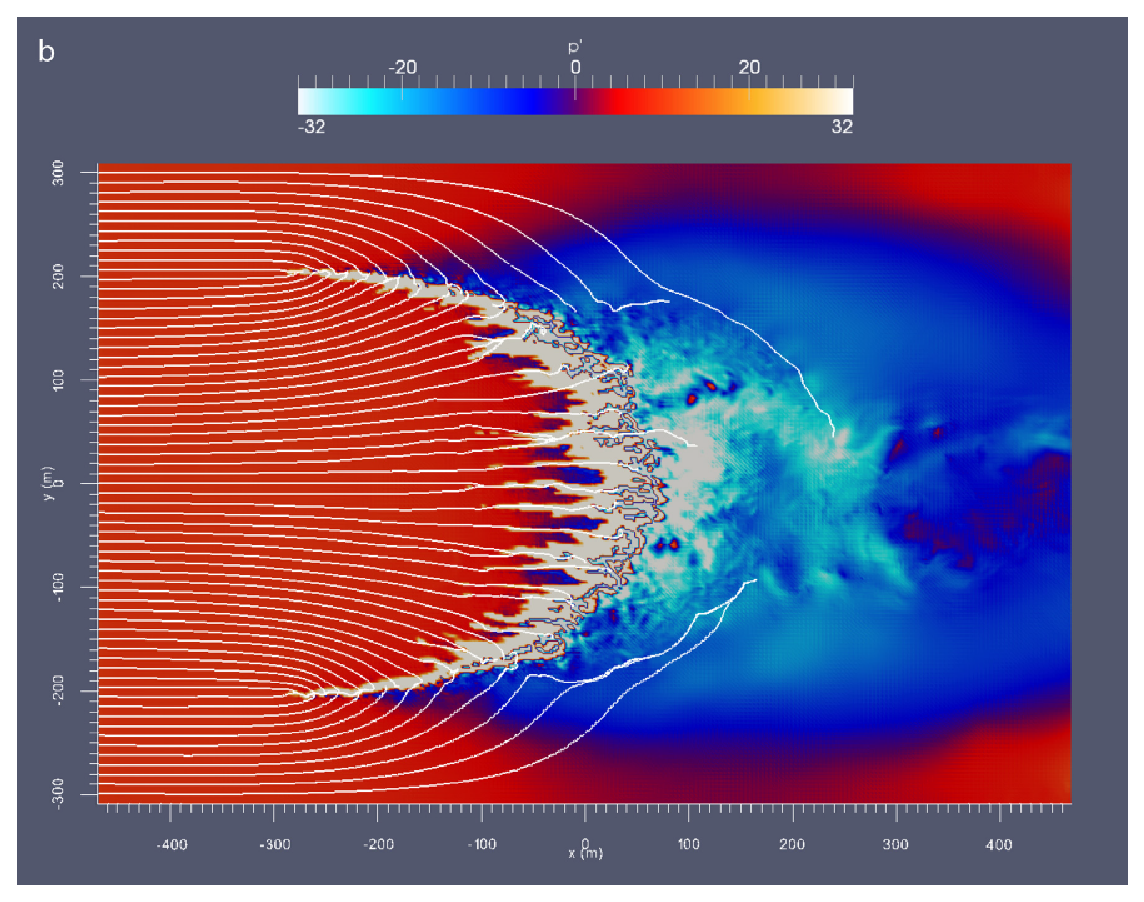
\includegraphics[height=0.1275\paperheight]{figures/CannfieldSinks}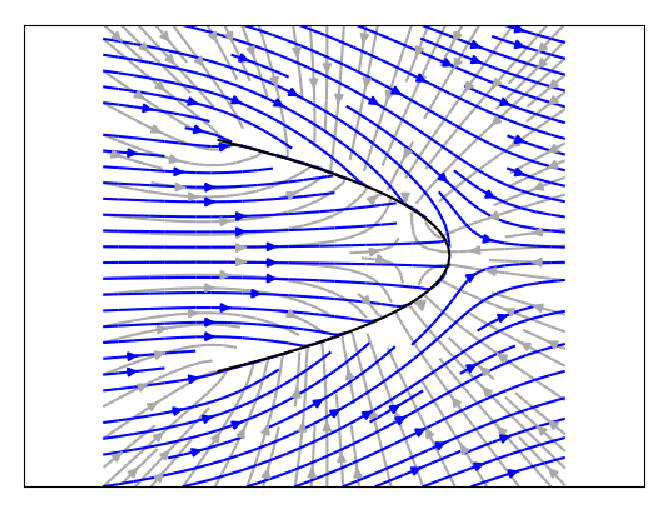
\includegraphics[height=0.13\paperheight]{figures/sinkBoth}}
\par\end{centering}
\small

\caption{A comparison of streamlines from a HIGRAD/FIRETEC \cite{linn1997firetec}
high-fidelity simulation (left) and streamlines from the interface
model (right). The streamlines of the convective sinks are plotted
in gray and the streamlines of $\lambda_{1}\vec{v}_{bg}+\lambda_{3}\vec{v}_{sink}$
$\left(\lambda_{1}=26.6;\lambda_{3}=1.0\right)$ are plotted in blue.
This figure demonstrates that with proper scaling of the convective
sink strength a similar velocity field to a high-fidelity model can
be attained.}
\end{wrapfigure}%

The larger a burning region the greater the heat released from combustion,
resulting in a stonger convective plume. For a fire with only a single
interior fireline the width is used as a way to scale the convective
sinks. The sum of all of these sinks with their strength, also scaled
by distance, forms the convective sink contribution to the interface
velocity. For firelines with multiple interior lines a Delauney triangulation
was used to mesh the interior burning region. The centers were used
as the sink locations and their strength scaled up by the corresponding
triangles area. The sum over these triangles and the same $r^{-1}$
distance scaling was used to form the convective sink velocity contribution
in these cases.

\subsection{Stability}

A numerical issue with modeling a fireline as a moving interface is
the distortion of the mesh as the interface moves. This leads to a
varying spatial resolution and can cause tangling and instabilities.
By using methods for curvature driven flow\cite{hou1994Ltheta} a
tangential velocity component is introduced that guarantees points
remain equispaced in arclength without affecting the shape of the
interface (Figure ). With this formulation, a well-behaved mesh is
attained and a larger number of stable timesteps can be taken. 

\subsubsection{L-$\theta$ Formulation}

With $\Gamma$ given by $X=\left(x\left(\alpha,t\right),y\left(\alpha,t\right)\right)$
a tangential velocity, $v_{s},$ is introduced to keep the points
along the intereface equispaced in arclength; $X_{t}=v_{n}\hat{n}\rightarrow X_{t}=v_{n}\hat{n}+v_{s}\hat{s}$,
where $\hat{s}$ is the unit tangent vector. To do this a switch of
parameterization of $\Gamma$ from \textit{x} and \textit{y} to the
tangent angle, $\theta,$ and arclength \textit{s}, more specifically
$\frac{\partial s}{\partial\alpha}$. With curvature driven flow $v_{n}=\kappa=\theta_{\alpha}/s_{\alpha}$
we can express the evolution of the curve in terms of $\theta$ and
$s_{\alpha}$via
\begin{equation}
s_{\alpha t}=\left(v_{s}\right)_{\alpha}-\frac{1}{s_{\alpha}}\theta_{\alpha}^{2}\label{eq:sAlphaT}
\end{equation}
\begin{equation}
\theta_{t}=\frac{1}{s_{\alpha}}\left(\frac{1}{s_{\alpha}}\theta_{\alpha}\right)_{\alpha}+\frac{v_{s}}{s_{\alpha}}\theta_{\alpha}.\label{eq:thetaT}
\end{equation}
 We can see that Eq. \ref{eq:thetaT} is an advection-diffusion equation
with stability condition $\Delta t<C\cdot\left(\bar{s_{\alpha}}h\right)^{2}$where
$\bar{s_{\alpha}=\min_{\alpha}s_{\alpha}}$ and \textit{h} is the
grid spacing in $\alpha.$ The stiffness of the problem comes through
Eq. (2) which can be dealt with by ensuring $s_{\alpha}$ doesn't
depend on $\alpha$. To achieve this enforce that $\frac{ds}{d\alpha}$
be everywhere equal to its mean
\[
s_{\alpha}(\alpha,t)=\frac{1}{2\pi}\int_{0}^{2\pi}s_{\alpha'}\left(\alpha^{'},t\right)d\alpha'=\frac{1}{2\pi}L(t)
\]
where $L(t)$ is the total length of the interface $\Gamma$. If $s_{\alpha}$
initially satisfies this constraint then 
\[
v_{s}(\alpha,t)=v_{s}(0,t)+\frac{2\pi}{L}\int_{0}^{\alpha}\theta_{\alpha'}^{2}d\alpha'-\frac{\alpha}{L}\int_{0}^{2\pi}\theta_{\alpha'}^{2}d\alpha',
\]
 resulting from IDONTKNOW, maintains the constraint in time. The tangential
velocity $v_{s}(0,t)$ is an arbitrary change of frame and can simply
be set to zero. Now $s_{\alpha}$ does not depend on $\alpha$ and
evolves with the length of the curve \textit{L}. Eqn. \ref{eq:sAlphaT}
now becomes an ODE for \textit{L} and we now have 
\begin{equation}
L_{t}=-\frac{1}{L}\int_{0}^{2\pi}\theta_{\alpha'}^{2}d\alpha'\label{eq:Lt'}
\end{equation}

\begin{equation}
\theta_{t}=\left(\frac{2\pi}{L}\right)^{2}\theta_{\alpha\alpha}+\frac{2\pi}{L}v_{s}\theta_{\alpha}.\label{eq:thetaT'}
\end{equation}

Substituting the curvature equation and it's derivative with respect
to $\alpha$ into Eqns. \ref{eq:Lt'} and \ref{eq:thetaT'} and using
the restriction $\int_{0}^{2\pi}s_{\alpha'}\left(\alpha^{'},t\right)d\alpha'=L(t)$
we can express our interface evolution in terms of the normal velocity
CITE MOORE
\begin{equation}
L_{t}=-\int_{0}^{2\pi}v_{n}\theta_{\alpha'}d\alpha'\label{eq:FinalLt}
\end{equation}

\begin{equation}
\theta_{t}=\frac{2\pi}{L}\left(v_{n}\right)_{\alpha}+\frac{2\pi}{L}v_{s}\theta_{\alpha}.\label{eq:FinalthetaT}
\end{equation}

\begin{wrapfigure}[18]{O}{0.55\columnwidth}%
\begin{centering}
\fbox{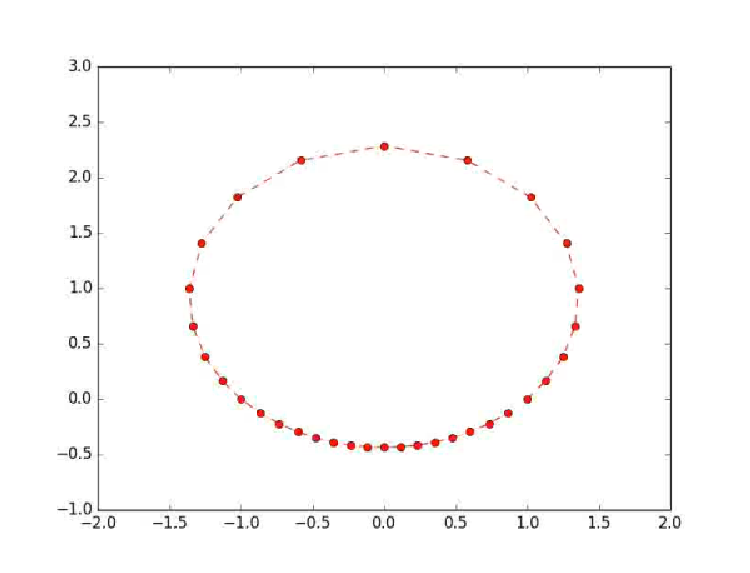
\includegraphics[width=0.2\paperwidth]{figures/noTheta}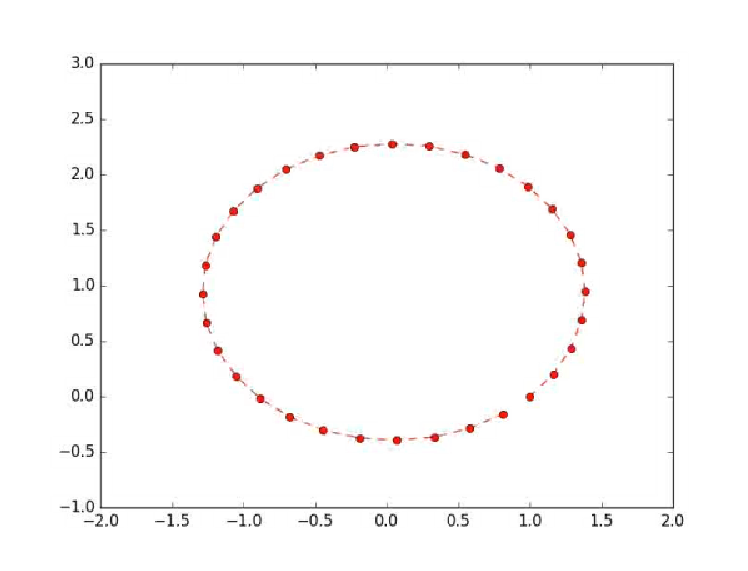
\includegraphics[width=0.2\paperwidth]{figures/Theta}}
\par\end{centering}
\small

\caption{Snapshots of two moving interfaces initialized as a unit circle centered
at the origin with $\vec{v}_{n}(t)=y\hat{n}$. The left interface
has no tangential velocity component and the right interface has the
tangential velocity implemented \cite{hou1994Ltheta}. Notice that
the right interface has the same shape as the left and keeps points
equispaced in arclength.}
\end{wrapfigure}%

Now $v_{n}$ can be formed using the methods described above section
and with Eqns. \ref{eq:FinalLt} and \ref{eq:FinalthetaT} the discretization
points can be kept equispaced in arclength. Since we are now keeping
track of opening angle and length we need to track a reference point
in cartesian space to account for translations of the interface. For
this we track the surface mean $\left\langle X\right\rangle $ which
moves according to 
\[
\left\langle X\right\rangle _{t}=\left\langle v_{n}\hat{n}+v_{s}\hat{s}\right\rangle 
\]
which is tracked using forward Euler\footnote{Explain this in more detail?}.

Show verification with just translation

Can do error convergence for translation tracking (not necessary)

Could have done optimization of streamline figure to determine lamda1
and lamda2 using firetec results to get time evolution of lambdas(if
they are constant proceed)

\section{Model Fitting}

In an effort to determine a limiting domain for $\lambda$ values
a Delayed-Rejection Adaptive-Metropolis Bayesian inference algorithm\cite{haario2006dram}
was used. 

The proposed model has unknown parameters that DRAM will identify.
The objective of DRAM is to start with a prescribed prior distribution
and then sample the parameter space to determine the posterior probability
density for each parameter. This is done by updating the likelihood
based on the error between the model and data. The DRAM algorithm
will show correlations between parameters, shortcomings of the model,
and quantify uncertainty. DRAM requires analysis of results and reinitialization
to attain good stationary posterior distributions. Depending on the
number of inferred parameters, the DRAM algorithm can require a large
amount of simulation runs to estimate these parameters, and my previous
experiences with HPC will prove useful. In addition, the computational
efficiency of this model makes it a natural fit for DRAM. 

The error that was used for driving the model took three points from
a head fire high fidelity simulation from HIGRAD/FIRETEC shown in
\cite{canfield2014numerical} which had the canonical parabolic fireline
shape I was hoping to capture. The initial fireline had a width (x
domain) of 20m and a height (y domain) of 100m, which was similar
to initial conditions in \cite{canfield2014numerical} with a backing
wind of 5 m/s in the positive x-direction. The points used for the
error were
\begin{center}
\begin{tabular}{|c|c|}
\hline 
x & y\tabularnewline
\hline 
\hline 
-30 & 0\tabularnewline
\hline 
544 & 0\tabularnewline
\hline 
{*} & 55\tabularnewline
\hline 
\end{tabular}
\par\end{center}

with the {*} being a free x value. Once a simulation was completed
the min and max x values and max y values were taken and compared
with the three points above. Since the initial fire line was initialized
with its center being on the x-axis with a background wind only in
the x-direction the developing fireline would be symmetric with respect
to the x-axis as well as not drift upward. This means that these points
were a consistent error measurement. 

There have been many improvements but there seems to be, for lack
of a better term, forbidden regions. There are combinations of $\lambda_{1},$
$\lambda_{2},$ and $\lambda_{3}$ that cause high frequency modes
developing and the interface breaks. This is an obvious obstacle when
using this model with DRAM since if a model returns nonsensical results
how does DRAM update the proposal distribution? Another layer of difficulty
is the fact that this code is written in Python. My solution for this
was to put catch points in my code to detect when the interface had
become unstable. When this happened the simulation was terminated
and a number code was returned instead of a result. In DRAM whenever
this code was received an error of $\infty$ was returned, which the
code is able to handle. My initial fix for this was making modifications
to a significant amount of the DRAM code to have it resample until
it received an actual result. This caused the time to get samples
to increase dramatically. I was able to do 200 runs over a 2 day period
which is a completely inadequate amount of samples to be able to do
any sort of analysis. By making the above change I was able to do
1,000 runs in a 1 day period. All of these runs returned dissappointing
results, although, there is some knowledge gained from using DRAM
with this model.

RESULTS
\begin{center}
\includegraphics[width=0.6\textwidth]{figures/chains1000}
\par\end{center}

Luckily this is the one that produced some possible information about
the model. From the bottom right plot we can see that there seems
to be an area where DRAM cannot sample. Taking a points from this
graph and fitting a line along the bottom region I arrived at an expression
of 
\[
13.846\lambda_{2}-\lambda_{3}\geq207.6
\]
for the bottom region. Running my simulation with parameters satisfying
this did in fact cause the simulation to break. Taking $\lambda_{1}$
and $\lambda_{2}$ factors from the upperleft plot and taking the
satisfying the negative of the above expression resulted in simulations
that ran the full time and didn't break. Sadly the simulation runs
resulting from the sampling means are not realistic. The final shape
of the resulting fireline does in fact have its width around the right
scale of the data points but it's height is much too large, \textasciitilde{}200m.
At least a rough constraint for stability for the model was able to
be realized. This exercise definitely has shown that much more foresight
needs to be used in order to utilize an MCMC sampling algorithm efficiently.

\bibliographystyle{plain}
\bibliography{References}


\section{SARndbox}

\section{Conclusion}
\end{document}
